\documentclass{my_eth_beamer}

\usepackage{my_math_eth}

\numberwithin{equation}{section}

% -----------------------------------------------------------------------------
% this document
\title{Introduction to Survey Sampling}
\newcommand{\TITLE}{Foundations}
\newcommand{\NR}{2}
\subtitle{Part \NR: \TITLE}
\author[Tobias Schoch]{Tobias Schoch}
\date{2026}

% -----------------------------------------------------------------------------
\begin{document}

\setstretch{1.1}

\section{\TITLE}\label{sec:basics}
\setcounter{section}{\NR}
\setcounter{Bsp}{1}

% -----------------------------------------------------------------------------
\begin{frame}
    \frametitle{Overview}
    \noindent \hspace{0.2em}\textcolor{fhnwblue}{\bfseries \NR~\TITLE}
    \begin{enumerate}[\NR.1]
        \item Sample and sampling design
        \item Probability sample
        \item Sample selection
        \item Randomization inference
        \item Asymptotics
    \end{enumerate}
\end{frame}

% -----------------------------------------------------------------------------
\begin{frame}
    \frametitle{\insertsectionnumber~\insertsection}
    A \alert{population} with $N$ elements can be represented by the
    \alert{finite} index set
    \begin{equation*}
        U = \{1, 2, \ldots, N\}.
    \end{equation*}
    \begin{itemize}
    \setlength{\itemsep}{4pt}
        \item The notation $U$ is derived from ``universe.''
        \item Each label $i$ ($i \in U$) can be assigned \alert{uniquely} to
            one unit.
    \end{itemize}
    The elements $i \in U$ have attributes or characteristics that can be
    recorded by \alert{variables}.
    \begin{itemize}
    \setlength{\itemsep}{4pt}
        \item Unless stated otherwise, we assume that all variables are
            \emph{real-valued}.
        \item They are \alert{not random variables}; their values are fixed.
    \end{itemize}
\end{frame}

% -----------------------------------------------------------------------------
\begin{frame}
    Let $y_i$ denote the variable of interest. The most important
    (population) \alert{characteristics} are
    \begin{align*}
        \ty &= \sum_{i \in U} y_i & \text{(population total)} \\[1em]
        \myu &= \frac{1}{N} \sum_{i \in U} y_i = \frac{\ty}{N} &
            \text{(population mean)}\\[1em]
        \sigma_y^2 &= \frac{1}{N - 1}\sum_{i \in U} (y_i - \myu)^2 &
            \text{(population variance).}
    \end{align*}
    \begin{itemize}
    \setlength{\itemsep}{8pt}
        \item Example: population total of all employees in retail trade
        \item Short notation: $t$ and $\sigma^2$
    \end{itemize}
\end{frame}

\subsection{Sample and sampling design}\label{sec:basics_sample}

% -----------------------------------------------------------------------------
\begin{frame}
    \frametitle{\insertsectionnumber.\insertsubsectionnumber~\insertsubsection}

    \begin{Def}[Sample]\label{def:sample}
        \vspace{-0.5em}
        A \alert{sample} $s$ is a \alert{subset} of $U$, formally
        $s \subseteq U$.
    \end{Def}

    \begin{itemize}
    \setlength{\itemsep}{8pt}
        \item Sets are unordered objects (they have no additional
            structure or ordering).
        \item Conceptual model: drawing numbered balls from an urn
            \alert{without replacement} (each element can occur at most once).
        \item \emph{Alternative definition}
            \vspace{0.25em}
            \begin{itemize}
            \setlength{\itemsep}{4pt}
                \item A sample (of size $n$) \emph{with replacement} can be
                    viewed as a \alert{sequence} or \alert{multiset}
                    $s = \{i_1, i_2, \ldots, i_n\}$, where
                    $i_k \in U$ for $k=1, \ldots, n$.
                \item In our finite-population setting, \alert{selecting the
                    same unit} more than once does not reveal an additional
                    population value.
            \end{itemize}
    \end{itemize}
\end{frame}

% -----------------------------------------------------------------------------
\begin{frame}
    \begin{itemize}
    \setlength{\itemsep}{8pt}
        \item We distinguish between \alert{probability} and
            \alert{nonprobability} sampling methods.
        \item In what follows, we focus on \alert{probability sampling} and
            probability samples \alert{without replacement}.
    \end{itemize}
    \vspace{1.5em}
    \textcolor{fhnwblue}{\bfseries Set of all possible samples}
    \vspace{0.5em}

    The \alert{set of all possible} samples from $U$ is defined as
    \begin{equation*}
        \samplespace := \{s : s \subseteq U\}.
    \end{equation*}

    \vspace{-1em}

    It contains:

    \begin{itemize}
    \setlength{\itemsep}{6pt}
        \item the empty set $\emptyset$ and the improper subset $U$;
            hence, $\samplespace$ is the power set and contains $2^N$
            elements,
        \item only samples in which each element can occur
            \emph{at most once}.
    \end{itemize}
\end{frame}

% -----------------------------------------------------------------------------
\begin{frame}
    \begin{Bsp}[U3]\label{ex:basics_u3}
        \vspace{-0.5em}
        For $U = \{1, 2, 3\}$, $\samplespace$ contains the following $2^3$
        subsets:
        \vspace{-0.5em}
        \begin{align*}
            s_0 &= \emptyset,\\
            s_1 &= \{1\}, & s_2 &= \{2\}, &s_3 &= \{3\},\\
            s_4 &= \{1, 2\},& s_5 &= \{1, 3\}, &s_6 &= \{2, 3\},
                &s_7 &= \{1, 2, 3\}.&
        \end{align*}
    \end{Bsp}
    The set of all possible samples from $U$ with \alert{fixed sample size}
    $n$ is given by
            \begin{equation*}
                \samplespace_n = \big\{s : s \subset U \; \text{and}
                \; \vert s \vert = n\big\}, \qquad (n > 0),
            \end{equation*}

    \vspace{-0.5em}

    and contains

    \vspace{-1.5em}

    \begin{equation*}
        \vert \samplespace_n \vert = \binom{N}{n} =
            \frac{N!}{n! \, (N - n)!}
    \end{equation*}

    \vspace{0.25em}

    \noindent distinct elements (i.e., individual samples).
\end{frame}

% -----------------------------------------------------------------------------
\begin{frame}
    For the discussion that follows, it is useful to introduce a
    \alert{quantity associated with the elements} $i \in s$.
    \vspace{0.5em}
    \begin{Def}[Sample inclusion indicator]
        Let $s$ be given. The \alert{sample inclusion indicator} is the
        indicator variable
        \begin{equation*}
            \indicator\{i \in s\} := \begin{cases}
                1 & \text{if}\; i \in s,\\
                0 & \text{otherwise,}
            \end{cases}
        \end{equation*}
        \noindent indicating whether an element $i \in U$ is included in the
        sample $s$ (short notation: $\indicator_i$).
    \end{Def}
    Remarks:
    \vspace{0.15em}
    \begin{itemize}
    \setlength{\itemsep}{5pt}
        \item Inclusion indicators allow us to write sample sums as sums over
            the entire population: $\sum_{i \in s} y_i = \sum_{i \in U}
            \indicator_i y_i$.
        \item This representation is particularly useful for derivations and
            proofs.
    \end{itemize}
\end{frame}

\subsection{Probability sample}\label{sec:basics_randomsample}

% -----------------------------------------------------------------------------
\begin{frame}
    \frametitle{\insertsectionnumber.\insertsubsectionnumber~\insertsubsection}
    \begin{Bsp}[Simple random sampling without replacement, SRS]\label{ex:basics_es}
        \vspace{-0.5em}
        Let $U$ be a population of size $N$. We want to select a (proper)
        sample $s$ of fixed size $n$ \alert{at random} from $U$
        (without replacement).
        \begin{itemize}
        \setlength{\itemsep}{8pt}
            \item There are $\vert \samplespace_n \vert = \binom{N}{n}$
                possible samples.
            \item Each sample $s$ has the same probability
            \begin{equation*}
                \frac{1}{\vert \samplespace_n \vert} = 1 \Big/ \binom{N}{n}
            \end{equation*}

            \vspace{-1em}

            \noindent of being selected.
        \item The above equation defines a \alert{discrete uniform
            distribution} (i.e., a probability distribution) on
                $\samplespace_n$.
        \end{itemize}
    \end{Bsp}
\end{frame}

% -----------------------------------------------------------------------------
\begin{frame}
    \begin{Def}[Probability distribution]\label{def:probmeasure}
        \vspace{-0.5em}
        Let $\samplespace$ denote the (finite, nonempty) set of all samples
        (sample space). We define a real-valued \alert{function}
        $\PP:\samplespace \rightarrow [0,1]$ that assigns a
        \alert{probability} to each \alert{elementary event} $\{s\}$, where
        $\PP$ satisfies the following properties:
        \begin{flalign*}
            1.& \; \PP\big(\{s\}\big) \geq 0, \quad \text{for every} \; s \in
                \samplespace, & \text{(nonnegativity)}\\[2em]
            2.& \; \sum_{s \in \samplespace} \PP\big(\{s\}\big) = 1.&
                \text{(normalization)}\\[1.5em]
            3.& \; \PP(E) := \sum_{s \in E: s \in
                \samplespace}\PP\big(\{s\}\big), \quad \text{for every
                subset $E$ of $\mathscr{S}$.} & \text{(additivity)}
        \end{flalign*}
    \end{Def}
\end{frame}

% -----------------------------------------------------------------------------
\begin{frame}
    We can now formulate three \emph{fundamental} definitions of classical
    survey sampling theory: the sampling design, the inclusion probability,
    and the probability sample.

    \vspace{1em}
    \begin{Def}[Sampling design]\label{def:design}
        \vspace{-0.5em}
        The mapping $p:\mathscr{S} \rightarrow [0,1]$, defined by
        $s \mapsto \PP(\{s\})$, is called a \alert{sampling design}
        (or simply design; also sampling plan).
    \end{Def}
    \vspace{0.75em}
    Remarks:
    \vspace{0.25em}
    \begin{itemize}
    \setlength{\itemsep}{8pt}
        \item We use $p$ for the design and write $p(s)$ for the probability
            of sample $s$ under design $p$.
        \item To distinguish between designs, we use subscripts, e.g.,
            $p_{\mSRS}$.
    \end{itemize}
\end{frame}

% -----------------------------------------------------------------------------
\begin{frame}
    The \alert{design}
    \begin{itemize}
    \setlength{\itemsep}{8pt}
        \item is the \alert{central element} of classical survey sampling
            theory (we will discuss this in more detail shortly);
        \item determines the \alert{sampling distribution} and therefore the
            stochastic properties of estimators (see Section
            2.\ref{sec:basics_randomization}).
    \end{itemize}

    \vspace{1.25em}

    \textcolor{fhnwblue}{\bfseries Why is the design central to survey
    sampling theory?}

    \vspace{0.25em}

    To answer this question, consider the \alert{freedom} we have in
    specifying a design. A design allows us to:
    \begin{enumerate}
    \setlength{\itemsep}{6pt}
        \item choose an \alert{arbitrary} set of possible samples to which
            we assign positive probability;
        \item distribute the total probability mass \alert{arbitrarily}
            across the samples (elements) in this set, subject to
            $\sum_{s \in \samplespace} p(s) = 1$.
    \end{enumerate}
\end{frame}

% -----------------------------------------------------------------------------
\begin{frame}
    \alert{We} are \alert{free}, within the framework of Definition
    \ref{def:design}, to specify a design for our purposes.
    \begin{itemize}
    \setlength{\itemsep}{4pt}
        \item The only \alert{constraints} arise from considerations of
            \alert{practicality} and \alert{optimality} (e.g., estimators
            with smaller variance).
        \item For example, we could specify a design that assigns a different
            probability to every possible sample (see Chapter 5).
    \end{itemize}
    \begin{Bsp}[U3, cont. of Ex. \ref{ex:basics_u3}]\label{ex:basics_u3_2}
        \vspace{-0.5em}
        Consider the design:
        \vspace{-1.5em}
        \begin{equation*}
            p_{U3}(s_k) = \begin{cases}
                    1/3 & \text{for} \; k = 4, 5 \;\text{and} \; 6\\
                    0 & \text{for} \; k = 0, 1, 2, 3 \; \text{and} \; 7.
                \end{cases}
        \end{equation*}
        \noindent Only samples of size $n = 2$ (i.e., $s_4 = \{1, 2\}$,
        $s_5 = \{1, 3\}$, and $s_6 = \{2, 3\}$) have a positive probability
        of being selected.
    \end{Bsp}
\end{frame}

\setcounter{Bsp}{\the\numexpr\value{Bsp}+1\relax}

% -----------------------------------------------------------------------------
\begin{frame}
    In addition to the probability $p(s)$ of a sample $s$, we are interested
    in the probability that an \alert{element} $i \in U$ is included in $s$.

    \vspace{0.5em}

    \begin{Def}[Inclusion probability]\label{def:inclusionprobabilities}
        \vspace{-0.5em}
        Let $p$ be given. The probability that \emph{element} $i$ is included
        in sample $s$ is called its (first-order sample) \alert{inclusion
        probability} and is given by
        \begin{equation*}
            \pi_i := \mathbb{P}(i \in s) = \sum_{s \, : \, i \in s} p(s)
                \qquad (i \in U),
        \end{equation*}
        where $\{s: i \in s\}$ is the set of all samples $s$ that contain
        element $i$.
    \end{Def}
\end{frame}

% -----------------------------------------------------------------------------
\begin{frame}
    \begin{Bsp}[U3, cont. of Ex. \ref{ex:basics_u3_2}]\label{ex:basics_u3_3}
        \vspace{-0.5em}
        Let $p_{U3}(s_k)$ be the design from Example
        \ref{ex:basics_u3_2}. Under this design, the samples
        \begin{equation*}
            s_4 = \{1, 2\}, \qquad s_5 = \{1, 3\} \qquad \text{and} \qquad
                s_6 = \{2, 3\}
        \end{equation*}
        \noindent are the only possible samples with positive probability
        $p_{U3}(s_k) = 1/3$, $k = 4, 5, 6$. It follows that the inclusion
        probabilities are $\pi_i = 2/3$ for every $i \in U$.
    \end{Bsp}
    \vspace{1em}
    \begin{Bsp}[\SRS, cont. of Ex. \ref{ex:basics_es}]\label{ex:basics_es_3}
        \vspace{-0.5em}
        Let $U$ be a population of size $N$. Under \alert{simple random
        sampling} (\SRS) of size $n$ ($0 < n < N$) from $U$,
        \begin{equation*}
            \pi_i = \frac{n}{N}, \qquad \text{for} \quad i \in U.
        \end{equation*}
    \end{Bsp}
\end{frame}

% -----------------------------------------------------------------------------
\begin{frame}
    \begin{itemize}
    \setlength{\itemsep}{8pt}
        \item The inclusion probabilities $\pi_i$ ($i \in U$) \alert{alone}
            do not fully characterize a design.
        \item Besides \SRS, for example,
            there are other designs that also yield inclusion probabilities
            $\pi_i = n/N$.
        \item A \alert{necessary and sufficient condition} for \SRS is that
            every possible sample $s$ has the same probability
            $p_{\mSRS}(s)$ of being selected.
        \item Using the inclusion probabilities, we can now give a
            \emph{common} definition of a probability sample (see, e.g.,
            Wikipedia).
    \end{itemize}

    \vspace{1em}

    \begin{Def}[Probability sample]\label{def:probsample}
        \vspace{-0.5em}
        In a \alert{probability sample}, every element $i \in U$ has a
        \alert{known} inclusion probability $\pi_i > 0$.
    \end{Def}
\end{frame}

% -----------------------------------------------------------------------------
\begin{frame}
    Remarks
    \vspace{0.25em}
    \begin{itemize}
    \setlength{\itemsep}{8pt}
        \item ``Known'' means that $\pi_i$ is available for every $i \in U$
            before the sample is selected.
        \item Using the $\pi_i$ \alert{together with knowledge of how} the
            sample is to be selected, or was selected, the design $p$ can
            generally be (re-)constructed. This is essential for statistical
            inference.
    \end{itemize}
\end{frame}

% -----------------------------------------------------------------------------
\begin{frame}
    \vspace{-0.25em}
    \begin{center}
        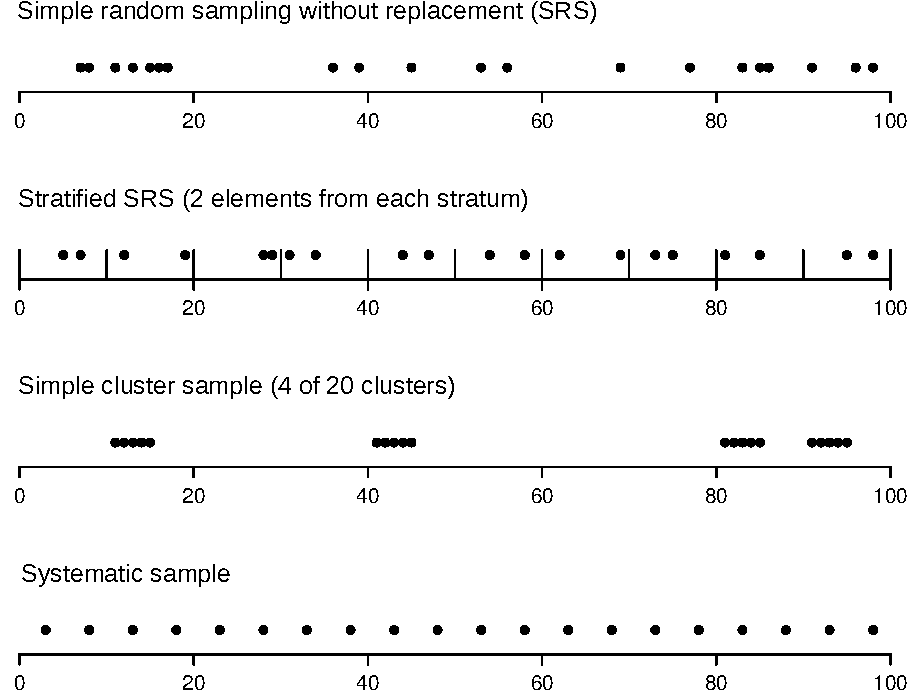
\includegraphics[width=0.7\textwidth]{figures/overview_en}
    \end{center}
\end{frame}

% -----------------------------------------------------------------------------
\begin{frame}
    \begin{enumerate}[1.]
    \setlength{\itemsep}{3pt}
        \item Population $U = \{1, \ldots, N\}$
        \item Sample space $\samplespace$ and sampling design $p$
            \begin{equation*}
                \samplespace \subseteq 2^U, \qquad p: \samplespace \to [0,1],
                \qquad \sum_{s \in \samplespace} p(s) = 1
            \end{equation*}

            \vspace{-1.5em}

            with

            \vspace{-0.5em}

            \begin{equation*}
                \PP_p(A) = \sum_{s \in A} p(s), \qquad A \subseteq \samplespace
                \qquad \text{(probability measure induced by $p$)}
            \end{equation*}
        \item Random sample $S$ and realization $s$
            \begin{equation*}
                S \in \samplespace, \qquad \PP_p(S = s) = p(s), \qquad
                    s \in \samplespace
            \end{equation*}
        \item Population elements $i$ and inclusion
            \begin{equation*}
                i \in U, \qquad \indicator_i = \indicator\{i \in S\}, \qquad
                    \pi_i = \PP_p(i \in S)
            \end{equation*}
    \end{enumerate}

    \begin{textblock}{4}(13.2,0.8)
        \textcolor{magenta}{\large{\textbf{Summary}}}
    \end{textblock}

\end{frame}

\subsection{Sample selection}\label{sec:basics_drawsample}

% -----------------------------------------------------------------------------
\begin{frame}
    \frametitle{\insertsectionnumber.\insertsubsectionnumber~\insertsubsection}
    \begin{itemize}
    \setlength{\itemsep}{8pt}
        \item For large populations, it is often impractical to enumerate all
            possible samples.
        \item A \alert{sampling scheme} (sampling algorithm) allows us to
            select a sample without enumerating all possible samples.
        \begin{itemize}
        \setlength{\itemsep}{4pt}
            \item A \alert{sequential} sampling scheme is a selection
                procedure applied to the list of units in $U$.
            \item For a fixed-size design with sample size $n$, the sample can
                be selected using a \alert{draw-by-draw sampling scheme}.
                At each of the $1,2,\ldots,n$ steps of the procedure, one unit
                is selected.
        \end{itemize}
       \item Many schemes and algorithms exist, e.g., eliminatory sampling
           and rejective algorithms; see \citet[][Chapter 3]{tille_2006}.
    \end{itemize}
\end{frame}

\setcounter{Bsp}{\the\numexpr\value{Bsp}+1\relax}

\subsection{Randomization inference}\label{sec:basics_randomization}

% -----------------------------------------------------------------------------
\begin{frame}
    \frametitle{\insertsectionnumber.\insertsubsectionnumber~\insertsubsection}
    \begin{itemize}
    \setlength{\itemsep}{10pt}
        \item \alert{Randomization inference} concerns the
            \alert{theoretical properties} of estimators under
            \alert{repeated sampling} under the same conditions.
        \item The main object of interest is the
            \alert{sampling distribution} of an estimator.
        \item In particular, it allows us to \alert{quantify the precision
            of an estimator}.
        \item Let $\theta_U$ denote the (population) characteristic of
            interest (e.g., population mean or total), and let
            $\widehat{\theta}$ be an estimator of $\theta_U$.
        \item We write $\widehat{\theta}(s)$ to emphasize that it is a
            \alert{statistic}.
    \end{itemize}
\end{frame}

% -----------------------------------------------------------------------------
\begin{frame}
    \begin{Def}[Expected value and variance]\label{def:expectation}
        \vspace{-0.5em}
        Let $p$ be given. The \alert{expected value} and \alert{variance}
        of the statistic $\widehat{\theta}(s)$ are defined as
        \begin{align*}
            \EE_p\big(\widehat{\theta}\,\big) & := \sum_{s \in \samplespace} p(s)
                \, \widehat{\theta}(s), && (\text{expected value}) \\[1em]
            \var_p\big(\widehat{\theta}\,\big) & := \sum_{s \in \samplespace}
                p(s) \, \big\{\widehat{\theta}(s) -
                \EE_p(\widehat{\theta}\,)\big\}^2. && (\text{variance})
        \end{align*}
    \end{Def}
    \vspace{0.25em}
    Remarks:
    \vspace{0.25em}
    \begin{itemize}
    \setlength{\itemsep}{6pt}
        \item Expected value and variance are taken \alert{over all possible
            samples} $s \in \mathscr S$ under the design $p$; we therefore also
            write $\EE_p$ and $\var_p$.
        \item Recall that $y_i$ ($i \in U$) are fixed quantities, not random
            variables. The sampling distribution arises \alert{exclusively}
            from the random selection of the sample.
    \end{itemize}
\end{frame}

% -----------------------------------------------------------------------------
\begin{frame}
    \begin{itemize}
    \setlength{\itemsep}{8pt}
        \item Expected value and variance can be used to define
            \alert{additional theoretical measures} of a sampling
            distribution.
    \end{itemize}
    \begin{align*}
        \bias_p(\widehat{\theta}\,) & := \EE_p\big(\widehat{\theta}\,\big) -
            \theta_U & \text{(bias)}\\[1.25em]
        \se_p\big(\widehat{\theta}\,\big) & :=
            \sqrt{\var_p\big(\widehat{\theta}\,\big)} &
            \text{(standard error)}\\[1.25em]
       \varcoef_p\big(\widehat{\theta}\,\big) & :=
            \frac{\se_p\big(\widehat{\theta}\,\big)}{\EE_p(\widehat{\theta}\,)},
            \quad \text{if} \;\, \EE_p(\widehat{\theta}\,) > 0 &
            \text{(coefficient of variation)}\\[1.25em]
        \MSE_p(\widehat{\theta}\,) & := \var_p(\widehat{\theta}\,) +
            \big\{\bias_p(\widehat{\theta}\,)\big\}^2 &
            \text{(mean squared error)}
    \end{align*}
\end{frame}

% -----------------------------------------------------------------------------
\begin{frame}
    \begin{itemize}
    \setlength{\itemsep}{10pt}
        \item An estimator $\widehat{\theta}$ is \alert{unbiased} for
            $\theta_U$ if
            \begin{equation*}
                \bias(\widehat{\theta}\,) = 0
                \qquad \text{equivalently} \qquad
                \EE(\widehat{\theta}\,) = \theta_U.
            \end{equation*}
        \item Let $\widehat{\theta}_1$ and $\widehat{\theta}_2$ be two unbiased
            estimators of $\theta_U$ under the same sampling design $p$.
            Estimator $\widehat{\theta}_1$ is \alert{more efficient} than
            $\widehat{\theta}_2$ if
            \begin{equation*}
                \var(\widehat{\theta}_1) < \var(\widehat{\theta}_2).
            \end{equation*}
        \item In most cases, an estimator
            $\widehat{\var}\big(\widehat{\theta}\,\big)$ of the variance
            $\var\big(\widehat{\theta}\,\big)$ can be constructed using only
            the sample data.
    \end{itemize}
\end{frame}

% -----------------------------------------------------------------------------
\begin{frame}
    To compare different sampling designs and their estimators, it is useful
    to introduce the concept of a strategy. Let $\theta_U$ denote the
    characteristic of interest.
    \vspace{0.25em}
    \begin{Def}[Strategy]\label{def:strategy}
        \vspace{-0.25em}
        A \alert{strategy} is a pair $(p, \widehat{\theta}\,)$ consisting of
        a sampling design $p$ and an estimator $\widehat{\theta}$ of
        $\theta_U$.
    \end{Def}
    \vspace{0.25em}
    Remarks:
    \vspace{0.25em}
    \begin{itemize}
    \setlength{\itemsep}{8pt}
        \item Example: $(p_{\mSRS}, \mys)$ denotes the sample mean
            $\mys = (1/n) \sum_{i \in s} y_i$ as an estimator of the
            population mean $\myu$ under \SRS of size $n$.
        \item Let $(p_1, \widehat{\theta}_1)$ and
            $(p_2, \widehat{\theta}_2)$ be two different (otherwise
            unspecified) strategies. We could, for example, use mean squared
            error to compare them.
    \end{itemize}
\end{frame}

\subsection{Asymptotics}\label{sec:basics_asymptotics}

% -----------------------------------------------------------------------------
\begin{frame}
    \frametitle{\insertsectionnumber.\insertsubsectionnumber~\insertsubsection}
    \begin{itemize}
    \setlength{\itemsep}{8pt}
        \item We have made \alert{no distributional assumptions} about the
            variable of interest $y_i$ ($i \in U$). Statistical inference
            therefore relies on \alert{approximation methods}.
        \item In classical statistics, the \alert{central limit theorem}
            (CLT) can be used to construct confidence intervals.
        \item The notion of asymptotics may seem incompatible with survey
            sampling from \emph{finite} populations. Indeed, it is impossible
            to let $n$ tend to infinity while keeping $N$ fixed.
        \item We therefore need a \alert{more elaborate asymptotic framework}
            in which $n_k,N_k \rightarrow \infty$ as $k \rightarrow \infty$.
    \end{itemize}
\end{frame}

% -----------------------------------------------------------------------------
\begin{frame}
    \begin{EinSatz}[H{\'a}jek, \citeyear{hajek_1960}]\label{thm:basics_clt}
        \vspace{-0.5em}
        Suppose that $n_k/N_k \rightarrow f \in (0,1)$ as
        $k \rightarrow \infty$. If the elements of the sequence
        $(y_i)_{i \in \mathbb{N}}$ satisfy
        \begin{equation}
            \lim_{k \rightarrow \infty} \frac{\max_{i \in U_k} (y_i -
                \widebar{y}_{U_k})^2}{\sum_{i \in U_k}
                (y_i - \widebar{y}_{U_k})^2} = 0,
                \tag{N}\label{eq:basics_noether}
        \end{equation}
        \noindent then, as $k \rightarrow \infty$,
        \begin{equation*}
            \frac{\widebar{y}_{s_k}
            -\widebar{y}_{U_k}}{\widehat{\se}\big(\widebar{y}_{s_k})} \;
            \dlim \; N(0, 1).
        \end{equation*}
    \end{EinSatz}
    \begin{itemize}
        \item $N(0,1)$ denotes the normal distribution with mean $0$ and
            variance $1$, and $\dlim$ denotes convergence in distribution
            (convergence in law).
        \item Condition (\ref{eq:basics_noether}) is called the Noether
            condition. It ensures that the variance is not dominated by a
            single observation $y_i$.
    \end{itemize}
\end{frame}

% -----------------------------------------------------------------------------
\begin{frame}
    \frametitle{\normalsize Confidence intervals}
    \begin{itemize}
    \setlength{\itemsep}{8pt}
        \item The CLT allows us to construct a \alert{confidence interval}
            (CI) for the population mean $\myu$ based on its \SRS estimator
            $\mys$, provided that $n$ is sufficiently large.
        \item A $100(1 - \alpha)\%$ confidence interval can be constructed as
            \begin{equation*}
                \mys \, \pm \, z_{1 - \alpha / 2} \, \widehat{\se}(\mys),
            \end{equation*}
            \noindent where $z_{1 - \alpha/2}$ is the
            $(1 - \alpha/2)$ quantile of the $N(0,1)$ distribution.
    \end{itemize}
\end{frame}

% -----------------------------------------------------------------------------
\begin{frame}
    \frametitle{Remarks}
    {\footnotesize
    \begin{itemize}
        \item \citet[][Chapters 1.2 and 1.3]{cassel_sarndal_etal_1977}
            define a sample in two different ways: the ``set case''
            (corresponding to our Definition \ref{def:sample}) and the
            ``sequence case'' (a sample defined as a sequence or multiset).
        \item Limit arguments and asymptotic properties of estimators and
            strategies are discussed in detail in
            \citet[][Chapter 1.3]{fuller_2009}.
        \item The theorem by H{\'a}jek cited above is a special case of
            Theorem 3.1 in \citet{hajek_1960}. In this special case, the
            Lindeberg condition is equivalent to the stated Noether
            condition; see \citet[][Remark 3.3]{hajek_1960}.
    \end{itemize}
    }
\end{frame}

% -----------------------------------------------------------------------------
\setcounter{section}{\the\numexpr\value{section}-1\relax}
\begin{frame}
    \frametitle{Literature}
    {\footnotesize
        \setstretch{1.1}
        \bibliographystyle{fhnw_en}
        \bibliography{master}
    }
\end{frame}

% -----------------------------------------------------------------------------
\lastpage

\end{document}
